\documentclass[a4paper,12pt]{article}
\usepackage[utf8]{inputenc}
\usepackage{amsmath}
\usepackage{amsfonts}
\usepackage{amssymb}
\usepackage{graphicx}
\numberwithin{equation}{section}

%opening
\title{Math Phys II HW4}
\author{Vince Baker}

\begin{document}

\maketitle

\section{Problem 1}
The series solutions of Bessel's equation are:
\begin{gather}
 J_n(x)=\sum_{k=0}^{\infty}\frac{(-1)^k}{k!\Gamma(n+k+1)}(\frac{x}{2})^{n+2k}\\
 J_{\frac{1}{2}}(x)=x^{\frac{1}{2}}\sum_{k=0}^{\infty}\frac{(-1)^kx^{2k}}{2^{2k+\frac{1}{2}}k!\Gamma(1+k+\frac{1}{2})}
\end{gather}
Since $\Gamma(x+1)=x\Gamma(x)$ and $\Gamma(\frac{1}{2})=\pi$, we can write the series:
\begin{gather}
 J_{\frac{1}{2}}(x)=\frac{(\frac{1}{2}x)^\frac{1}{2}}{\frac{1}{2}\pi}
 -\frac{(\frac{1}{2}x)^\frac{5}{2}}{1!\frac{3}{2}\frac{1}{2}\pi}
 +\frac{(\frac{1}{2}x)^\frac{9}{2}}{2!\frac{5}{2}\frac{3}{2}\frac{1}{2}\pi}\\
 J_{\frac{1}{2}}(x)=\frac{(\frac{1}{2}x)^\frac{1}{2}}{\frac{1}{2}\pi}(1-\frac{x^2}{3!}+\frac{x^4}{5!}\ldots)\\
 J_{\frac{1}{2}}(x)=\sqrt{\frac{2}{\pi x}}\sin x
\end{gather}
For $n=-\frac{1}{2}$, the series is:
\begin{gather}
 J_{-\frac{1}{2}}=\frac{(\frac{1}{2}x)^{-\frac{1}{2}}}{\sqrt{\pi}}(1-\frac{x^2}{2!}+\frac{x^4}{4!}-\ldots)=\sqrt{\frac{2}{\pi x}}\cos x
\end{gather}
The first two terms can now bootstrap the recurrence relation $J_{n+1}=\frac{2n}{x}J_n-J_{n-1}$.
Ignoring the constants in front of $J_{-\frac{1}{2}}$ and $J_{\frac{1}{2}}$, we have:
\begin{gather}
 J_{\frac{3}{2}}=\frac{1}{\sqrt{x^3}}\sin x- \frac{1}{\sqrt{x}}\cos x=\frac{1}{\sqrt{x}}(\frac{\sin x}{x}-\cos x)\\
 J_{\frac{5}{2}}=\frac{3}{x\sqrt{x}}(\frac{\sin x}{x}-\cos x)-\frac{1}{\sqrt{x}}\sin x= \frac{1}{\sqrt{x}}(3(\frac{\sin x}{x^2}-\frac{\cos x}{x} )-\sin x)
\end{gather}
\\
When the Bessel series expansion of $f(x)=\sum_{k=1}^{\infty}a_kJ_m(\alpha_{mk}x)$ we prove Parseval's relation:
\begin{equation}
 \int_0^1|f(x)|^2xdx=\frac{1}{2}\sum_{k=1}^{\infty}a_k^2|J_{m+1}(\alpha_{mk})|^2
\end{equation}
We substitute the Bessel series into the LHS of the equation and swap the integration and sum. 
The integration range and weighting function are correct for an orthonormal Bessel basis.
All terms with $k\neq m$ will vanish by orthogonality. We are left with:
\begin{gather}
 I=\sum_{k=1}^{\infty}a_k^2\int_0^1(J_m(\alpha_{mk}x))^2xdx\\
 I=\frac{1}{2}\sum_{k=1}^{\infty}a_k^2(J_{m+1}(\alpha_{mk}))^2
\end{gather}

\section{Problem 2}
We solve the diffusion equation for the temperature in a long cylinder:
\begin{gather}
 \nabla^2T=\frac{1}{\kappa}\frac{\partial T}{\partial t}
\end{gather}
The temporal solution has the form $e^{-k^2\kappa t}$ with separation constant $k^2$.
In cylindrical coordinates the spatial solution has the form:
\begin{gather}
 T=\sum_{\ell,m,n=0}^{\infty}a_{\ell mn}J_m(n\rho)e^{-im\phi}e^{-\ell z}
\end{gather}
With an infinitely long cylinder and axial symmetry we have $\ell=m=0$ and $n^2=K^2$.
The solution has the form:
\begin{gather}
 T=\sum_{k=1}^{\infty}a_{k}J_0(k\rho )e^{-\kappa kt}
\end{gather}
We now apply the boundary condition $T(\rho =b)=0$. This forces $kb=\alpha_{0k},\ k=\frac{\alpha_{0k}}{b}$.
We can now apply the boundary condition that the cylinder is at temperature $T_0$ at $t=0$ to solve for the coefficients.
\begin{gather}
 T_0=\sum_{k=1}^{\infty}a_kJ_0(\frac{\alpha_{0k}}{b}\rho)\\
 a_k=\frac{1}{A_m}\int_{0}^{b}T_0 J_0(\frac{\alpha_{0k}}{b}\rho)\rho d\rho\\
 A_m=\frac{b^2}{2}J_{1}^2(\alpha_{0k})\\
 a_k=\frac{2T_0}{b^2J_{1}^2(\alpha_{0k})}\int_{0}^{b}J_0(\frac{\alpha_{0k}}{b}\rho)\rho d\rho
\end{gather}
At the center of the cylinder $(\rho=0)$ the integral is $\frac{b^2}{2}$, so the solution is:
\begin{gather}
 T(0,t)=\sum_{k=1}^{\infty}   \frac{T_0}{J_{1}^2(\alpha_{0k})}  e^{\frac{-\alpha_{0k}^2\kappa t}{b^2}}
\end{gather}
With $t\gg \frac{b^2}{\kappa}$ the behavior will be determined by the smallest values of $\alpha_{0k}$ as everything else will fall off exponentially faster.
So in this limit the solution is $\approx \frac{T_0}{J_{1}^2(\alpha_{01})}e^{-\alpha_{01}t}$.
\\

\section{Problem 3}
We solve for the potential inside a sphere composed of two insulated, charged hemispheres.
The hemispheres are held at potential $\pm V_0$ and we take the symmetric axis along $\theta=0$.
Laplace's equation with axial symmetry has the solutions:
\begin{gather}
 \sum_{\ell=0}^{\infty}(a_\ell r^\ell+b_\ell r^{-\ell-1} )P_\ell(cos \theta)
\end{gather}
We are looking for interior solutions so all the $b_\ell$ are 0 since they are singular at the origin.
\begin{gather}
 \sum_{\ell=0}^{\infty}(a_\ell r^\ell )P_\ell(cos \theta)
\end{gather}
We now apply the boundary conditions at $r=R_0$ and solve for the coefficients of the Legendre expansion.
\begin{gather}
 f(R_0,\theta)=\sum_{\ell=0}^{\infty}a_\ell R_0^{\ell}P_\ell(\cos \theta)\\
 a_\ell R_0^\ell=\frac{2\ell + 1}{2}\int_{-1}^{1}f(R_0,\theta)P_\ell(u) du\\
  a_\ell R_0^\ell=V_0\frac{2\ell + 1}{2}[\int_{0}^{1} P_\ell(u) du- \int_{-1}^{0} P_\ell(u) du ]\\
\end{gather}
The even Legendre integrals will cancel, and we are left with the series:
\begin{gather}
 a_\ell=\frac{V_0}{2}[2+\frac{3}{R_0}-\frac{7}{4R_0^3}+\frac{11}{8R_0^5}+\ldots]
\end{gather}
We can now write the interior solution:
\begin{gather}
 \Phi(r,\theta)=\frac{V_0}{2}[2P_0(\cos \theta)+\frac{3r}{R_0}P_1(\cos \theta)-\frac{7r^3}{4R_0^3}P_3(\cos \theta)+\frac{11r^5}{8R_0^5}P_5(\cos \theta)+\ldots]
\end{gather}
\\
We now find the exterior solution with a time-dependent driving potential $\pm V_0e^{i\omega t}$ on the two hemispheres.
The general solution for the exterior solution of the Helmholtz equation with axial symmetry is:
\begin{gather}
 \Phi(r,\theta)=\sum_{\ell}(a_{\ell}h_{\ell}(kr))P_{\ell}(\cos \theta)
\end{gather}
Where $H_{ell}$ is a substitute for a combination of both spherical Henkel functions.
Imposing the boundary condition and solving the same Legendre expansion as above we find:
\begin{gather}
 \Phi(R_0,\theta, t) = f(r,\theta, t)\\
 a_{\ell}=\frac{V_0}{2}e^{-i\omega t}[\frac{2}{h_0(kR_0)}+\frac{3}{h_1(kR_0)}-\frac{7}{4h_3(kR_0)}+\ldots]\\
 \begin{aligned}
 \Phi(r,\theta,t)=\frac{V_0}{2}e^{-i\omega t}[\frac{2}{h_0(kR_0)}h_0(kr)P_0(\cos \theta)+ \\
	      \frac{3}{h_1(kR_0)}h_1(kr)P_1(\cos \theta)-\\ 
	      \frac{7}{4h_3(kR_0)}h_3(kr)P_3(\cos \theta)+\ldots]
 \end{aligned}
\end{gather}
As $r\rightarrow \infty$ the spherical Henkel functions approach $\frac{e^{ikr}}{r}$. 
We can then write the far field solution as:
\begin{gather}
  \begin{aligned}
 \Phi(r,\theta,t)=\frac{V_0}{2r}e^{i(kr-\omega t)}[\frac{2}{h_0(kR_0)}P_0(\cos \theta)+ \\
	      \frac{3}{h_1(kR_0)}P_1(\cos \theta)-\\ 
	      \frac{7}{4h_3(kR_0)}P_3(\cos \theta)+\ldots]
 \end{aligned}
\end{gather}


\section{Problem 4}
We find the mutual electrostatic potential energy of the two 1s electrons in a hydrogen atom.
The 1s wavefunctions are $\psi(r)=\sqrt{\frac{8}{\pi a_0^3}}e^{\frac{-2r}{a_0}}$.
The mutual potential energy is given by:
\begin{gather}
 U=\int\int\psi^*(r_1)\psi^*(r_2)\frac{e^2}{r_{12}}\psi(r_1)\psi(r_2) d^3r_1 d^3r_2
\end{gather}
We expand $\frac{1}{r_{12}}$ in spherical harmonics. 
Since the wavefunctions have no anglar dependence only a constant factor of $16\pi$ will survive the angular integral.
We can now collect the constant terms $K=(\sqrt{\frac{8}{\pi a_0^3}})^4e^216\pi^2$ and write the integral:
\begin{gather}
 U=K \int_{0}^{R} r_1^2 e^{\frac{-4r_1}{a_0}}dr_1\{\int_{0}^{r_1} r_2^2\frac{ e^{\frac{-4r_2}{a_0}} }{r_1} dr_2
 + \int_{r_1}^{R} r_2 e^{\frac{-4r_2}{a_0}}  dr_2\}\\
 U=K \int_{0}^{R} r_1^2 e^{\frac{-4r_1}{a_0}}dr_1\{\ (\frac{a_0^2}{16}-\frac{a_0}{8} )e^{\frac{-4r_1}{a_0}} 
 -\frac{a_0^3}{32r_1}(e^{\frac{-4r_1}{a_0}}-1 )-e^{\frac{-4R}{a_0}}(\frac{a_0^2}{16}+\frac{a_0}{4}R) \}
\end{gather}
Wolfram Alpha says this integral is:\\
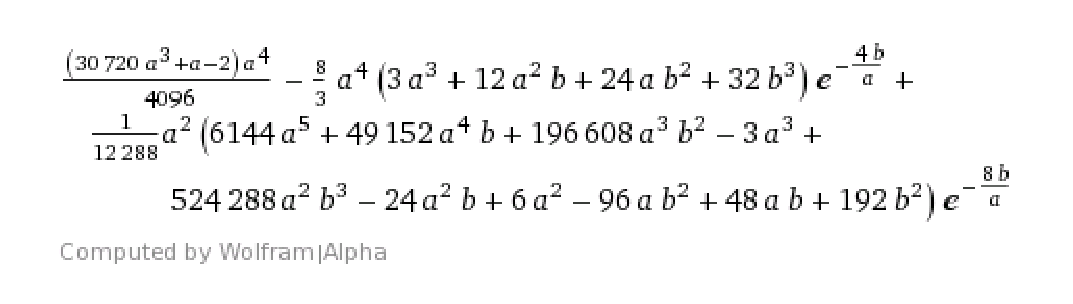
\includegraphics{BigEq2}
\\
Where $a=a_0,\ b=R$.



\end{document}
